% Options for packages loaded elsewhere
\PassOptionsToPackage{unicode}{hyperref}
\PassOptionsToPackage{hyphens}{url}
\PassOptionsToPackage{dvipsnames,svgnames,x11names}{xcolor}
%
\documentclass[
  letterpaper,
  DIV=11,
  numbers=noendperiod]{scrreprt}

\usepackage{amsmath,amssymb}
\usepackage{iftex}
\ifPDFTeX
  \usepackage[T1]{fontenc}
  \usepackage[utf8]{inputenc}
  \usepackage{textcomp} % provide euro and other symbols
\else % if luatex or xetex
  \usepackage{unicode-math}
  \defaultfontfeatures{Scale=MatchLowercase}
  \defaultfontfeatures[\rmfamily]{Ligatures=TeX,Scale=1}
\fi
\usepackage{lmodern}
\ifPDFTeX\else  
    % xetex/luatex font selection
\fi
% Use upquote if available, for straight quotes in verbatim environments
\IfFileExists{upquote.sty}{\usepackage{upquote}}{}
\IfFileExists{microtype.sty}{% use microtype if available
  \usepackage[]{microtype}
  \UseMicrotypeSet[protrusion]{basicmath} % disable protrusion for tt fonts
}{}
\makeatletter
\@ifundefined{KOMAClassName}{% if non-KOMA class
  \IfFileExists{parskip.sty}{%
    \usepackage{parskip}
  }{% else
    \setlength{\parindent}{0pt}
    \setlength{\parskip}{6pt plus 2pt minus 1pt}}
}{% if KOMA class
  \KOMAoptions{parskip=half}}
\makeatother
\usepackage{xcolor}
\setlength{\emergencystretch}{3em} % prevent overfull lines
\setcounter{secnumdepth}{5}
% Make \paragraph and \subparagraph free-standing
\ifx\paragraph\undefined\else
  \let\oldparagraph\paragraph
  \renewcommand{\paragraph}[1]{\oldparagraph{#1}\mbox{}}
\fi
\ifx\subparagraph\undefined\else
  \let\oldsubparagraph\subparagraph
  \renewcommand{\subparagraph}[1]{\oldsubparagraph{#1}\mbox{}}
\fi


\providecommand{\tightlist}{%
  \setlength{\itemsep}{0pt}\setlength{\parskip}{0pt}}\usepackage{longtable,booktabs,array}
\usepackage{calc} % for calculating minipage widths
% Correct order of tables after \paragraph or \subparagraph
\usepackage{etoolbox}
\makeatletter
\patchcmd\longtable{\par}{\if@noskipsec\mbox{}\fi\par}{}{}
\makeatother
% Allow footnotes in longtable head/foot
\IfFileExists{footnotehyper.sty}{\usepackage{footnotehyper}}{\usepackage{footnote}}
\makesavenoteenv{longtable}
\usepackage{graphicx}
\makeatletter
\def\maxwidth{\ifdim\Gin@nat@width>\linewidth\linewidth\else\Gin@nat@width\fi}
\def\maxheight{\ifdim\Gin@nat@height>\textheight\textheight\else\Gin@nat@height\fi}
\makeatother
% Scale images if necessary, so that they will not overflow the page
% margins by default, and it is still possible to overwrite the defaults
% using explicit options in \includegraphics[width, height, ...]{}
\setkeys{Gin}{width=\maxwidth,height=\maxheight,keepaspectratio}
% Set default figure placement to htbp
\makeatletter
\def\fps@figure{htbp}
\makeatother
\newlength{\cslhangindent}
\setlength{\cslhangindent}{1.5em}
\newlength{\csllabelwidth}
\setlength{\csllabelwidth}{3em}
\newlength{\cslentryspacingunit} % times entry-spacing
\setlength{\cslentryspacingunit}{\parskip}
\newenvironment{CSLReferences}[2] % #1 hanging-ident, #2 entry spacing
 {% don't indent paragraphs
  \setlength{\parindent}{0pt}
  % turn on hanging indent if param 1 is 1
  \ifodd #1
  \let\oldpar\par
  \def\par{\hangindent=\cslhangindent\oldpar}
  \fi
  % set entry spacing
  \setlength{\parskip}{#2\cslentryspacingunit}
 }%
 {}
\usepackage{calc}
\newcommand{\CSLBlock}[1]{#1\hfill\break}
\newcommand{\CSLLeftMargin}[1]{\parbox[t]{\csllabelwidth}{#1}}
\newcommand{\CSLRightInline}[1]{\parbox[t]{\linewidth - \csllabelwidth}{#1}\break}
\newcommand{\CSLIndent}[1]{\hspace{\cslhangindent}#1}

\KOMAoption{captions}{tableheading}
\makeatletter
\@ifpackageloaded{tcolorbox}{}{\usepackage[skins,breakable]{tcolorbox}}
\@ifpackageloaded{fontawesome5}{}{\usepackage{fontawesome5}}
\definecolor{quarto-callout-color}{HTML}{909090}
\definecolor{quarto-callout-note-color}{HTML}{0758E5}
\definecolor{quarto-callout-important-color}{HTML}{CC1914}
\definecolor{quarto-callout-warning-color}{HTML}{EB9113}
\definecolor{quarto-callout-tip-color}{HTML}{00A047}
\definecolor{quarto-callout-caution-color}{HTML}{FC5300}
\definecolor{quarto-callout-color-frame}{HTML}{acacac}
\definecolor{quarto-callout-note-color-frame}{HTML}{4582ec}
\definecolor{quarto-callout-important-color-frame}{HTML}{d9534f}
\definecolor{quarto-callout-warning-color-frame}{HTML}{f0ad4e}
\definecolor{quarto-callout-tip-color-frame}{HTML}{02b875}
\definecolor{quarto-callout-caution-color-frame}{HTML}{fd7e14}
\makeatother
\makeatletter
\makeatother
\makeatletter
\@ifpackageloaded{bookmark}{}{\usepackage{bookmark}}
\makeatother
\makeatletter
\@ifpackageloaded{caption}{}{\usepackage{caption}}
\AtBeginDocument{%
\ifdefined\contentsname
  \renewcommand*\contentsname{Tabla de contenidos}
\else
  \newcommand\contentsname{Tabla de contenidos}
\fi
\ifdefined\listfigurename
  \renewcommand*\listfigurename{Listado de Figuras}
\else
  \newcommand\listfigurename{Listado de Figuras}
\fi
\ifdefined\listtablename
  \renewcommand*\listtablename{Listado de Tablas}
\else
  \newcommand\listtablename{Listado de Tablas}
\fi
\ifdefined\figurename
  \renewcommand*\figurename{Figura}
\else
  \newcommand\figurename{Figura}
\fi
\ifdefined\tablename
  \renewcommand*\tablename{Tabla}
\else
  \newcommand\tablename{Tabla}
\fi
}
\@ifpackageloaded{float}{}{\usepackage{float}}
\floatstyle{ruled}
\@ifundefined{c@chapter}{\newfloat{codelisting}{h}{lop}}{\newfloat{codelisting}{h}{lop}[chapter]}
\floatname{codelisting}{Listado}
\newcommand*\listoflistings{\listof{codelisting}{Listado de Listados}}
\makeatother
\makeatletter
\@ifpackageloaded{caption}{}{\usepackage{caption}}
\@ifpackageloaded{subcaption}{}{\usepackage{subcaption}}
\makeatother
\makeatletter
\@ifpackageloaded{tcolorbox}{}{\usepackage[skins,breakable]{tcolorbox}}
\makeatother
\makeatletter
\@ifundefined{shadecolor}{\definecolor{shadecolor}{rgb}{.97, .97, .97}}
\makeatother
\makeatletter
\makeatother
\makeatletter
\makeatother
\ifLuaTeX
\usepackage[bidi=basic]{babel}
\else
\usepackage[bidi=default]{babel}
\fi
\babelprovide[main,import]{spanish}
% get rid of language-specific shorthands (see #6817):
\let\LanguageShortHands\languageshorthands
\def\languageshorthands#1{}
\ifLuaTeX
  \usepackage{selnolig}  % disable illegal ligatures
\fi
\IfFileExists{bookmark.sty}{\usepackage{bookmark}}{\usepackage{hyperref}}
\IfFileExists{xurl.sty}{\usepackage{xurl}}{} % add URL line breaks if available
\urlstyle{same} % disable monospaced font for URLs
\hypersetup{
  pdftitle={Análisis Estadístico (UA)},
  pdfauthor={Joaquín Bermejo; Victorio Costa},
  pdflang={es},
  colorlinks=true,
  linkcolor={blue},
  filecolor={Maroon},
  citecolor={Blue},
  urlcolor={Blue},
  pdfcreator={LaTeX via pandoc}}

\title{Análisis Estadístico (UA)}
\author{Joaquín Bermejo \and Victorio Costa}
\date{2024-06-23}

\begin{document}
\maketitle
\ifdefined\Shaded\renewenvironment{Shaded}{\begin{tcolorbox}[interior hidden, borderline west={3pt}{0pt}{shadecolor}, sharp corners, breakable, boxrule=0pt, frame hidden, enhanced]}{\end{tcolorbox}}\fi

\renewcommand*\contentsname{Tabla de contenidos}
{
\hypersetup{linkcolor=}
\setcounter{tocdepth}{2}
\tableofcontents
}
\bookmarksetup{startatroot}

\hypertarget{prefacio}{%
\chapter*{Prefacio}\label{prefacio}}
\addcontentsline{toc}{chapter}{Prefacio}

\markboth{Prefacio}{Prefacio}

Desde la cátedra de Análisis Estadístico, les damos una cálida
bienvenida a este nuevo curso, donde nos sumergiremos nuevamente en el
fascinante mundo de los datos, la toma de decisiones y, sobre todas las
cosas, el apasionante proceso de aprendizaje.

¿Alguna vez se han preguntado cómo las empresas líderes toman decisiones
cruciales basadas en datos? ¿O cómo pueden prever tendencias económicas
que transforman industrias enteras? A lo largo de este curso,
exploraremos técnicas y conceptos fundamentales que nos permitirán
descubrir el valioso conocimiento que los datos pueden brindarnos. Desde
los conceptos básicos de la teoría de probabilidad hasta métodos
gráficos e inferenciales, aprenderemos a resolver problemas y ofrecer
soluciones basadas en un análisis riguroso.

¡Esperamos que tomen este recorrido como un desafío, como una
oportunidad para poner a prueba sus habilidades y construir un espacio
interactivo donde tanto ustedes como nosotros enriquezcamos nuestros
conocimientos!

\bookmarksetup{startatroot}

\hypertarget{herramientas-de-conteo}{%
\chapter{Herramientas de conteo}\label{herramientas-de-conteo}}

\hypertarget{introducciuxf3n}{%
\section{Introducción}\label{introducciuxf3n}}

Las \textbf{herramientas de conteo} sirven para contar el número de
maneras distintas de obtener un cierto resultado, incluso bajo algunas
condiciones o restricciones. Algunos ejemplos son:

\begin{itemize}
\tightlist
\item
  conociendo a los 3 ganadores de una competencia pero sin saber el
  orden en que ganaron, determinar de cuántas formas distintas podría
  haberse formado un podio entre esos 3 participantes.
\item
  contar el número de formas en el que 5 personas pueden viajar en un
  auto de 5 asientos, considerando que sólo dos de ellas tienen licencia
  de conducir.
\item
  contar el número de partidas de ajedrez que pueden jugarse en un
  torneo con 32 participantes, bajo la condición de que cada par de
  participantes se enfrenten una y sólo una vez.
\item
  contar el número de estados posibles en los que puede hallarse un cubo
  de Rubik.
\item
  contar el número de formas en el que 200 invitados a una fiesta pueden
  organizarse en mesas de 6 personas. Considerar cómo este número se
  vería afectado si a la fiesta asisten dos personas que se detestan y
  no quieren sentarse en la misma mesa.
\item
  sabiendo que en WhatsApp se recibieron 23 mensajes de 5 chats, contar
  el número de formas en que estos 23 mensajes podrían encontrarse
  repartidos entre esos 5 chats.
\end{itemize}

\hypertarget{herramientas-de-conteo-simples}{%
\section{Herramientas de conteo
simples}\label{herramientas-de-conteo-simples}}

\hypertarget{factoriales}{%
\subsection{Factoriales}\label{factoriales}}

El caso más simple para contar resultados posibles, del cual se
desprenden todos los demás, consiste en contar de cuántas maneras puede
reordenarse un conjunto de \(n\) elementos, siendo \(n\) un número
natural (es decir, \(n \in \mathbb{N}\)).

\begin{examplebox}

\begin{center}
\textbf{Ejemplo 1}

\end{center}

Tres personas (las llamaremos \(A\), \(B\) y \(C\)) quieren sentarse en
un sofá de tres asientos. ¿De cuántas formas distintas pueden hacerlo?

\textbf{Solución:} Este caso es lo suficientemente sencillo como para
resolverlo por \emph{enumeración exhaustiva}: se pueden listar todos los
resultados posibles y después contar el tamaño de dicha lista.

Los posibles reordenamientos de un grupo de 3 personas son:

\begin{flexcenter}

\begin{half}

\begin{longtable}[]{@{}lll@{}}
\toprule\noalign{}
\endhead
\bottomrule\noalign{}
\endlastfoot
\(ABC\) & \(BAC\) & \(CAB\) \\
\(ACB\) & \(BCA\) & \(CBA\) \\
\end{longtable}

\end{half}

\end{flexcenter}

Por lo tanto, existen 6 formas de que tres personas se sienten en un
sillón de tres asientos.

\end{examplebox}

El problema con la enumeración exhaustiva es que el número de
reordenamientos crece rápidamente a medida que el tamaño del conjunto (o
sea, \(n\)) aumenta. Si logramos hallar un patrón o una fórmula en la
forma de contar el número de reordenamientos posibles, entonces podremos
calcular el número de reordenamientos para cualquier \(n\), sin tener
que enumerar todos los casos posibles.

\begin{tcolorbox}[enhanced jigsaw, opacitybacktitle=0.6, breakable, toptitle=1mm, toprule=.15mm, colback=white, coltitle=black, leftrule=.75mm, colframe=quarto-callout-tip-color-frame, left=2mm, opacityback=0, bottomrule=.15mm, arc=.35mm, colbacktitle=quarto-callout-tip-color!10!white, bottomtitle=1mm, titlerule=0mm, title=\textcolor{quarto-callout-tip-color}{\faLightbulb}\hspace{0.5em}{Idea clave}, rightrule=.15mm]

Las herramientas de conteo nos permiten contar elementos sin necesidad
de enumerarlos.

\end{tcolorbox}

Volvamos al ejemplo con \(n=3\). Para empezar: ¿cuántas personas
distintas pueden sentarse en el primer asiento del sofá? Es evidente que
cualquiera de las tres personas en cuestión (\(A\), \(B\) y \(C\))
pueden ocupar este lugar y por lo tanto la respuesta es 3. Ahora bien,
¿cuántas personas pueden sentarse en el segundo asiento, si consideramos
que ya hay una persona sentada en el primero? Las opciones se ven
reducidas. Si bien no sabemos quién, una de las personas ya está sentada
en el primer asiento y por lo tanto no es elegible para sentarse en el
segundo asiento. Sólo las dos personas restantes pueden ocupar dicho
lugar y en consecuencia la respuesta es 2. Por último, ¿cuántas personas
pueden sentarse en el tercer asiento si los dos primeros ya están
ocupados? En este caso la respuesta es trivial: si dos de las tres
personas ya se encuentran sentadas, entonces sólo queda una persona para
sentarse en el tercer asiento y en consecuencia la respuesta es 1.

En resumen, existen 3 posibilidades distintas para el primer asiento;
por cada una de ellas se tienen 2 posibilidades distintas para el
segundo asiento; a su vez, por cada una de las combinaciones anteriores
(una persona en el primer asiento y otra en el segundo asiento) se
tiene, por descarte, una sola posibilidad para el tercer asiento.

En total se tienen
\[3 \times 2 \times 1 = 6 \;\text{resultados posibles.}\]

¿Qué pasaría si fuesen \(n=4\) personas en un sofá de 4 asientos? Si
llamamos \(D\) a la cuarta persona, la tabla de resultados posibles para
esta situación es:

\begin{flexcenter}

\begin{half}

\begin{longtable}[]{@{}llll@{}}
\toprule\noalign{}
\endhead
\bottomrule\noalign{}
\endlastfoot
\(ABCD\) & \(BACD\) & \(CABD\) & \(DABC\) \\
\(ABDC\) & \(BADC\) & \(CADB\) & \(DACB\) \\
\(ACBD\) & \(BCAD\) & \(CBAD\) & \(DBAC\) \\
\(ACDB\) & \(BCDA\) & \(CBDA\) & \(DBCA\) \\
\(ADBC\) & \(BDAC\) & \(CDAB\) & \(DCAB\) \\
\(ADCB\) & \(BDCA\) & \(CDBA\) & \(DCBA\) \\
\end{longtable}

\end{half}

\end{flexcenter}

Nuevamente, por enumeración exhaustiva podemos ver que hay 24 resultados
posibles para esta situación. ¿Cómo podríamos haberlo deducido sin tener
que listar cada resultado? Afortunadamente, el razonamiento para el caso
\(n=4\) es análogo al caso \(n=3\).

Cualquier persona puede sentarse en el primer asiento y por lo tanto hay
4 formas distintas en las que este lugar puede ser ocupado. Para cada
uno de esos escenarios, cualquiera de las tres personas restantes puede
ocupar el segundo asiento, resultando en 3 formas posibles de ocuparlo.
A su vez, para cada una de las combinaciones anteriores (una persona en
el primer asiento y otra persona en el segundo asiento) cualquiera de
las dos personas restantes puede ocupar el tercer asiento y por lo tanto
se tienen 2 formas posibles de ocuparlo. Finalmente, si tres de las
cuatro personas ya se encuentran sentadas en los primeros tres asientos
del sofá, entonces sólo queda un escenario posible para el cuarto
asiento: que sea ocupado por la persona restante.

En total se tienen
\[4 \times 3 \times 2 \times 1 = 24 \;\text{resultados posibles.}\]

Es fácil ver que este razonamiento es aplicable a cualquier número de
personas y asientos. En general, si se tienen \(n\) personas queriendo
sentarse en un sofá de \(n\) asientos, existen
\[n \times (n-1) \times (n-2) \times \cdots \times 3 \times 2 \times 1\]
formas distintas de lograrlo.

El procedimiento anterior es utilizado con frecuencia en
combinatoria\footnote{La combinatoria es la rama de las matemáticas que
  estudia la enumeración de configuraciones que satisfacen ciertas
  condiciones.} y por lo tanto tiene su propio símbolo y nombre.

Sea \(n \in \mathbb{N}\), se llama \textbf{factorial de} \(\mathbf{n}\)
a
\[n! = n \times (n-1)  \times (n-2) \times \cdots \times 3 \times 2 \times 1\]

Existen dos formas alternativas de definir el factorial de \(n\): en
forma iterativa y en forma recursiva.

Forma iterativa:
\[n = \prod_{i=1}^n i = 1 \times 2 \times 3 \times \cdots \times (n-1) \times n\]

Forma recursiva:
\[n! = n \times (n-1)! \qquad \forall \; n \in \mathbb{N}\]

Un detalle a tener en cuenta con la forma recursiva es que para \(n=1\)
se tiene que \(1! = 1 \times 0!\). Por convención, se considera que
\(0! = 1\).

\begin{examplebox}

\begin{center}
\textbf{Ejemplo 2}

\end{center}

Una lista de reproducción de Spotify está compuesta por 9 canciones. ¿En
cuántos órdenes distintos pueden escucharse todas las canciones de la
lista?

\textbf{Solución:} El problema consiste en averiguar cuántos
reordenamientos son posibles para la lista de 9 canciones. Como ya
vimos, esto equivale a
\[9! = 9 \times 8 \times 7 \times 6 \times 5 \times 4 \times 3 \times 2 \times 1 = 362\,880 \text{ órdenes distintos.}\]

\end{examplebox}

Nótese el gran número de reordenamientos que resulta de un número tan
pequeño de elementos. Este número es tan grande que sería inviable
resolver el problema por enumeración exhaustiva. Incluso para una lista
de 5 canciones se tendrían \(5!=120\) posibles reordenamientos, los
cuales ya son muchos como para escribirlos uno por uno. En líneas
generales, el número factorial crece muy rápidamente, incluso más que el
número exponencial.

\begin{figure}

{\centering 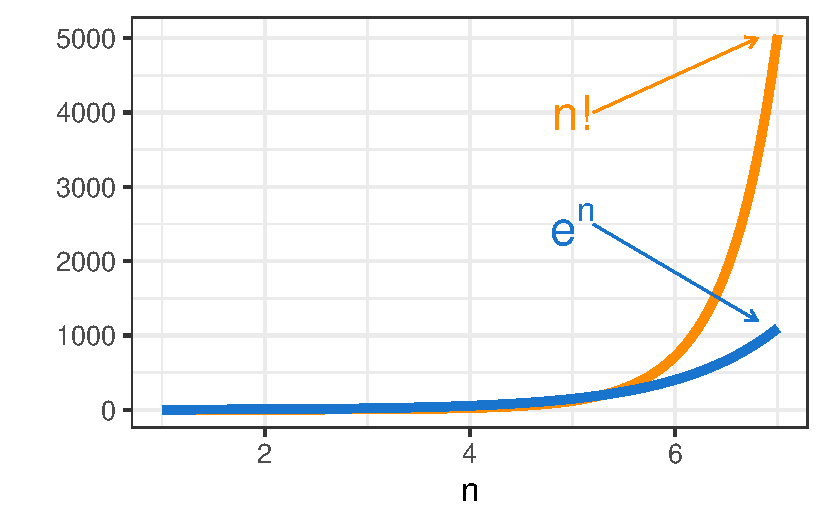
\includegraphics{conteo_files/figure-pdf/fig-crecimiento-factorial-1.pdf}

}

\caption{\label{fig-crecimiento-factorial}Comparación de las funciones
exponencial y factorial.}

\end{figure}

Como ya se dijo, el factorial es la base de las herramientas de conteo,
pero no es la única. Es una forma práctica de contar el número de
reordenamientos de \(n\) elementos. Por ejemplo, en una carrera de
Fórmula 1, donde compiten 20 autos, podemos usar el factorial para
contar el número de resultados distintos para dicha carrera. Pero ¿qué
pasaría si sólo nos interesara el resultado del podio, es decir, de las
primeras 3 posiciones? Dicho de otro modo, dado un conjunto de \(n\)
elementos, ¿cómo podemos contar el número de \emph{subconjuntos
ordenados} de \(r<n\) elementos?

\hypertarget{permutaciones}{%
\subsection{Permutaciones}\label{permutaciones}}

Intentemos resolver el problema propuesto en la sección anterior
aplicando la misma lógica que nos llevó a descubrir el número factorial.

\begin{examplebox}

\begin{center}
\textbf{Ejemplo 3}

\end{center}

En una carrera de Fórmula 1 compiten 20 vehículos. ¿De cuántas formas
distintas puede establecerse un podio en dicha carrera?

\textbf{Solución:} Cualquiera de los 20 conductores es elegible para
ocupar el primer puesto. A su vez, por cada una de estas posibilidades,
quedan 19 conductores que podrían tomar el segundo puesto. Finalmente,
teniendo ya un conductor en el primer puesto y otro conductor en el
segundo puesto, cualquiera de los 18 conductores restantes pueden ocupar
el tercer puesto.

En conclusión, existen
\[20 \times 19 \times 18 = 6\,840 \text{ podios posibles.}\]

\end{examplebox}

Ignorando el contexto del problema, acabamos de deducir la forma de
contar el número de subconjuntos ordenados de tamaño \(r=3\) obtenidos a
partir de un conjunto de tamaño \(n=20\).

Para resolver este ejemplo empleamos la misma técnica de
``multiplicación descendente'' que dedujimos para el factorial, pero
esta vez nos detuvimos después de \(r\) factores en lugar de multiplicar
los \(n\) primeros números naturales. ¿Cómo podríamos generalizar este
procedimiento en una fórmula?

Para valores \(n\) y \(r\) cualesquiera (con \(r<n\)), el cálculo
realizado es
\[n \times (n-1) \times (n-2) \times \cdots \times (n-r+2) \times (n-r+1)\]

Al ser un producto, multiplicar el valor anterior por 1 no lo modifica
en absoluto. Pero si escribimos ese 1 como
\(\textstyle\frac{(n-r)!}{(n-r)!}\) entonces se obtendría
\[n \times (n-1) \times \cdots \times (n-r+1) \times \frac{(n-r)!}{(n-r)!} = \frac{n \times (n-1) \times \cdots \times (n-r+1) \times (n-r)!}{(n-r)!}\]

Utilizando la definición recursiva del número factorial, el producto de
los dos últimos factores del numerador equivale a \((n-r+1)!\) y por lo
tanto la expresión anterior equivale a
\[\frac{n \times (n-1) \times \cdots \times (n-r+2) \times (n-r+1)!}{(n-r)!}\]

A su vez, el producto de los dos últimos factores del numerador en esta
nueva expresión equivale a \((n-r+2)!\). Aplicando sucesivamente este
procedimiento se llega a que el numerador es igual a \(n!\). Es decir,
la expresión anterior equivale a \[\frac{n!}{(n-r)!}\]

Hemos deducido otra herramienta de conteo importante.

Sean \(n \in \mathbb{N}_0, \; r \in \mathbb{N}_0\) \footnote{El conjunto
  \(\mathbb{N}_0\) equivale al conjunto de números naturales y el número
  0, es decir que
  \(\mathbb{N}_0 = \{0\} \cup \mathbb{N} = \{ 0,1,2,3,4,\cdots \}\). Si
  bien los casos donde \(n=0\) y/o \(r=0\) son triviales y poco
  frecuentes en la práctica, estos son posibles desde el punto de vista
  matemático y por lo tanto se los incluye. Esto no significa que no
  tienen sentido práctico: el caso \(r=0\), por ejemplo, refiere al
  número de formas de elegir subconjuntos de cero elementos; se
  considera que sólo hay una forma posible de hacer esto (no elegir
  ningún elemento).} tales que \(r \leq n\), se llama
\textbf{permutación de} \(\mathbf{n}\) elementos en \(\mathbf{r}\) a
\[_nP_r = \frac{n!}{(n-r)!}\]

Nótese que cuando \(r=n\) se tiene
\[_nP_n = \frac{n!}{(n-n)!} = \frac{n!}{0!} = \frac{n!}{1} = n!\]

Esto tiene sentido, visto que lo que estamos contando a través de este
número es el número de subconjuntos ordenados de tamaño \(n\) obtenidos
a partir de un conjunto de tamaño \(n\). Esto no es más que el número de
reordenamientos entre \(n\) elementos, lo cual (por lo visto en la
sección anterior) sabemos que equivale a \(n!\). En otras palabras, el
número de reordenamientos de un conjunto de \(n\) elementos no es más
que un caso particular de una permutación. Es por ello que el número de
reordenamientos de conjuntos de tamaño \(n\) suele denominarse
\textbf{permutación de} \(\mathbf{n}\) elementos y simbolizarse como
\(P_n\).

\begin{examplebox}

\begin{center}
\textbf{Ejemplo 4}

\end{center}

Se tienen 8 franjas de tela, cada una de un color diferente. Se pretende
utilizar tres de ellas para armar una bandera compuesta por una franja
superior, una franja media y una franja inferior. ¿Cuántas banderas
distintas son posibles?

\textbf{Solución:} Partiendo de un conjunto de \(n=8\) elementos,
debemos calcular el número de subconjuntos ordenados de tamaño \(r=3\).
Es decir, debemos calcular una permutación de 8 en 3.
\[_8P_3 = \frac{8!}{5!} = 8 \times 7 \times 6 = 336 \text{ banderas posibles.}\]

\end{examplebox}

\begin{tcolorbox}[enhanced jigsaw, opacitybacktitle=0.6, breakable, toptitle=1mm, toprule=.15mm, colback=white, coltitle=black, leftrule=.75mm, colframe=quarto-callout-warning-color-frame, left=2mm, opacityback=0, bottomrule=.15mm, arc=.35mm, colbacktitle=quarto-callout-warning-color!10!white, bottomtitle=1mm, titlerule=0mm, title=\textcolor{quarto-callout-warning-color}{\faExclamationTriangle}\hspace{0.5em}{Advertencia}, rightrule=.15mm]

Más allá de que una permutación se defina como un cociente de
factoriales, en la práctica no es aconsejable calcular dicho cociente.
Esto es porque los factoriales tienden a ser números muy grandes; tanto
es así que es muy fácil encontrarse con números cuyo factorial es
imposible de calcular con la tecnología de la que hoy
disponemos.\footnotemark{} Incluso si pudiésemos calcular los números
factoriales que componen el cociente, éstos podrían ser extremadamente
grandes, dificultando considerablemente los cálculos. \footnotemark{} Es
por esto que, de hacerse los cálculos a mano, se recomienda seguir el
proceso de multiplicación descendente.

\end{tcolorbox}

\footnotetext{En las calculadoras convencionales el mayor número
factorial que puede calcularse es \(69!\), mientras que en las
computadoras actuales dicho número es \(170!\).}

\footnotetext{\url{https://www.youtube.com/watch?v=flqC3c2wsNI}}

\begin{tcolorbox}[enhanced jigsaw, opacitybacktitle=0.6, breakable, toptitle=1mm, toprule=.15mm, colback=white, coltitle=black, leftrule=.75mm, colframe=quarto-callout-warning-color-frame, left=2mm, opacityback=0, bottomrule=.15mm, arc=.35mm, colbacktitle=quarto-callout-warning-color!10!white, bottomtitle=1mm, titlerule=0mm, title=\textcolor{quarto-callout-warning-color}{\faExclamationTriangle}\hspace{0.5em}{Advertencia}, rightrule=.15mm]

Si bien hablamos de subconjuntos ordenados, al calcular permutaciones no
es importante que exista una verdadera ordinalidad entre los elementos
(en el sentido de que uno de ellos anteceda o suceda a otro), sino en
realidad que estos sean distinguibles entre sí. Claramente la
ordinalidad es una condición suficiente para lograr lo anterior, pero no
es una condición necesaria, como veremos en el ejemplo siguiente.

\end{tcolorbox}

\begin{examplebox}

\begin{center}
\textbf{Ejemplo 5}

\end{center}

El club de debate de una escuela secundaria cuenta con nueve miembros.
La semana próxima se realizará un torneo de debate que tomará lugar en
cuatro ciudades diferentes: Seattle, Baltimore, Washington y Denver. El
director de la escuela debe elegir a un participante para enviar a cada
ciudad. ¿De cuántas formas distintas puede hacer esto?

\textbf{Solución:} Nótese que en este ejemplo importa no sólo cuaĺes de
los 9 miembros del club son seleccionados, sino también a qué ciudad es
enviado cada uno. Se fija entonces el orden de las ciudades tal como
fueron enumeradas en el enunciado, de modo que el primer participante
será enviado a Seattle; el segundo, a Baltimore; el tercero, a
Washington y el cuarto, a Denver. Nótese que el orden elegido para las
ciudades no afecta los cálculos. Efectivamente, para cualquier orden
arbitrario entre las 4 ciudades se obtendría el mismo resultado.

Hay 9 posibles participantes para ser enviados al torneo en Seattle. Por
cada uno de ellos, cualquiera de los 8 restantes puede ser enviado a
Baltimore. A su vez, por cada par de participantes elegidos para Seattle
y Baltimore respectivamente, cualquiera de los 7 restantes puede ser
asignado a Washington. Por último, para cualquier terna ordenada de tres
alumnos, cualquiera de los 6 restantes puede ser enviado a Denver.

Por lo tanto, se tienen
\[_9P_5 = 9 \times 8 \times 7 \times 6 = 3\,024 \text{ formas posibles.}\]

\end{examplebox}

Este ejemplo plantea un escenario donde cada uno de los participantes
seleccionados es asignado a una ciudad diferente y por lo tanto los
cuatro roles son distinguibles entre sí. Supongamos ahora que el torneo
de debate se lleva a cabo en un solo lugar, y por lo tanto los cuatro
roles son equivalentes e intercambiables. Ciertamente esto llevaría a
una reducción en el número de formas distintas de elegir los
participantes, porque soluciones que anteriormente podían considerarse
distintas (por ejemplo, el conjunto de alumnos \([A, B, C, D]\) y el
conjunto \([B, D, A, C]\)) ahora deberían contarse como una única
solución.

La pregunta es: ¿cuál es entonces el número de formas distintas de
elegir los participantes?

\hypertarget{combinaciones}{%
\subsection{Combinaciones}\label{combinaciones}}

\begin{examplebox}

\begin{center}
\textbf{Ejemplo 6}

\end{center}

Un club de debate de con nueve miembros debe elegir a cuatro de ellos
para representar a su escuela en un torneo nacional. ¿De cuántas formas
distintas puede hacerse esto?

\textbf{Solución:} Por lo visto en el Ejemplo 5 sabemos que, si cada uno
de los cuatro puestos a ocupar fuese diferenciable de los otros tres,
habría \(_9P_4 = 3\,024\) formas distintas de lograr el objetivo. Pero
ahora estos puestos son todos iguales y por lo tanto sólo importa cuáles
de los nueve alumnos ingresan en la selección, sin importar el orden en
que se los elige. Esto implica que el resultado será menor al del
Ejemplo 5. Procedamos a calcular este valor.

Supongamos que el conjunto total de alumnos es
\(\{ A,B,C,D,E,F,G,H,I \}\). Un subconjunto posible de tamaño \(r=4\) es
\(\{ B, E, G, H \}\). El valor \(_9P_4\) cuenta este mismo subconjunto
varias veces, porque permuta sus elementos y considera dichas
permutaciones como resultados distintos. En particular ¿cuántas veces
cuenta cada uno? Sabemos que la cantidad de permutaciones entre 4
elementos es igual a \(P_4 = 4! = 24\). Es decir que por cada 24
subconjuntos enumerados por el valor \(_9P_4\), ahora sólo nos interesa
uno.

En conclusión, se tienen
\[\frac{_9P_4}{4!} = \frac{3024}{24} = 126 \text{ formas posibles.}\]

\end{examplebox}

En general, dado un conjunto de \(n\) elementos, hay
\(\textstyle\frac{_nP_r}{r!}\) formas distintas de elegir
\emph{subconjuntos no ordenados} de \(r \leq n\) elementos. Este cálculo
corresponde a nuestra tercer herramienta de conteo.

Sean \(n \in \mathbb{N}_0, \; r \in \mathbb{N}_0\) tales que
\(r \leq n\), se llama \textbf{combinación de} \(\mathbf{n}\) elementos
en \(\mathbf{r}\) a
\[_nC_r = \frac{_nP_r}{r!} = \frac{n!}{r! \, (n-r)!}\]

Nótese que
\(_nC_r \leq \; _nP_r \quad \forall \; n, r \in \mathbb{N}_0\) tales que
\(r \leq n\).

En otras palabras, cuando queramos contar el número de ``grupos'' (de
tamaño fijo) que pueden formarse a partir de un conjunto, utilizaremos
combinaciones. Si adicionalmente nos interesa establecer ``roles''
dentro de dicho grupo, utilizaremos permutaciones.

\begin{examplebox}

\begin{center}
\textbf{Ejemplo 7a}

\end{center}

Un comité de 3 personas debe formarse a partir de un grupo de 20
personas. ¿De cuántas formas distintas puede hacerse esto?

\textbf{Solución:} Tenemos un conjunto de tamaño \(n=20\) y nos interesa
armar un grupo de tamaño \(r=3\), pero sin asignar roles dentro del
grupo (es decir, los 3 cargos a ocupar son indistinguibles entre sí). En
conclusión, debemos usar una combinación:
\[_{20}C_3 = \frac{20!}{3!\;17!} = \frac{20 \times 19 \times 18}{3 \times 2 \times 1} = 1\,140 \text{ comités posibles.}\]

\begin{center}\rule{0.5\linewidth}{0.5pt}\end{center}

\begin{center}
\textbf{Ejemplo 7b}

\end{center}

Supongamos ahora que los 3 cargos a ocupar en el comité son presidente,
vicepresidente y secretario. ¿Cómo afecta esto el número de posibles
comités?

\textbf{Solución:} Como ahora los cargos son distinguibles entre sí, ya
no importa únicamente quiénes son las 3 personas seleccionadas sino
también el rol que ocupa cada una de ellas. Debemos usar entonces una
permutación:
\[_{20}P_3 = \frac{20!}{17!} = 20 \times 19 \times 18 = 6\,840 \text{ comités posibles.}\]

\end{examplebox}

\hypertarget{herramientas-de-conteo-con-repeticiuxf3n}{%
\section{Herramientas de conteo con
repetición}\label{herramientas-de-conteo-con-repeticiuxf3n}}

Las herramientas presentadas hasta ahora tienen una importante
limitación: asumen que cada elemento de nuestro conjunto original sólo
puede ser seleccionado una única vez. En los ejemplos vistos hasta ahora
esta suposición es adecuada: si necesitamos llenar 3 cupos para formar
un comité, no tendría sentido darle 2 cargos a la misma persona (por
ejemplo: que sea presidente y vicepresidente simultáneamente). Estos son
casos donde la selección se realiza \emph{sin repetición} o \emph{sin
reposición}. Es análogo al bingo: cada vez que se saca una bola, ésta no
vuelve al bolillero y por lo tanto su correspondiente número no puede
ser seleccionado otra vez.

Pero existen casos donde amerita realizar una \textbf{selección
\emph{con repetición}} o \emph{con reposición}. En la analogía del
bingo, esto sería equivalente a extraer una bola, anotar su número
correspondiente y volver a meterla en el bolillero, de modo que dicha
bola podría volver a ser seleccionada en extracciones posteriores.

Cuando la selección es con repetición, las fórmulas que vimos hasta
ahora ya no sirven. Esto es porque \textbf{el número de subconjuntos
posibles aumenta} cuando pasamos de una selección sin repetición a una
con repetición. Veámoslo con un ejemplo.

\begin{examplebox}

\begin{center}
\textbf{Ejemplo 8}

\end{center}

Tenemos una bolsa con tres bolas enumeradas del 1 al 3. Se procede a
hacer una selección con repetición de dos bolas; es decir, se selecciona
una primera bola, se anota su número, se la vuelve a introducir en la
bola y se selecciona una segunda bola. Si nos interesa distinguir la
primera bola de la segunda, ¿cuántas extracciones distintas son
posibles?

\textbf{Solución:} Si la selección fuese sin repetición, habría
\(_3P_2 = 6\) formas posibles de seleccionar dos bolas. Estas son:

\begin{flexcenter}

\begin{half}

\begin{longtable}[]{@{}lll@{}}
\toprule\noalign{}
\endhead
\bottomrule\noalign{}
\endlastfoot
\((1,2)\) & \((2,1)\) & \((3,1)\) \\
\((1,3)\) & \((2,3)\) & \((3,2)\) \\
\end{longtable}

\end{half}

\end{flexcenter}

Pero como la selección es con repetición, también debemos contar los
casos donde se selecciona dos veces la misma bola. Estos son 3 casos en
total: \((1,1)\), \((2,2)\) y \((3,3)\). Por lo tanto, en total se
tienen: \[_3P_2 + 3 = 6 + 3 = 9 \text{ extracciones posibles.}\]

\end{examplebox}

En conclusión, debemos deducir nuevas fórmulas para las permutaciones y
combinaciones en los casos donde se selecciona con repetición.

\hypertarget{permutaciones-con-repeticiuxf3n}{%
\subsection{Permutaciones con
repetición}\label{permutaciones-con-repeticiuxf3n}}

Supongamos que tenemos una bolsa con \(n=7\) canicas y debemos
seleccionar \(r=3\) de ellas. Anteriormente, bajo el paradigma de una
selección sin repetición, nuestra lógica era la siguiente: hay 7 formas
de seleccionar la primera canica, luego 6 formas de seleccionar la
segunda (porque la primera que seleccionamos ya no está disponible) y
por último 5 formas de seleccionar la tercera (porque tanto la primera
como la segunda canica seleccionada ya no están disponibles). En total,
existen \(7 \times 6 \times 5 = 210\) formas distintas de realizar esta
selección.

Ahora bien, bajo una selección con repetición, esta falta de
disponibilidad que considerábamos luego de cada selección ya no existe,
porque la reposición actúa como un \emph{reset} y entonces todas las
canicas están disponibles en todas las extracciones. ¿Cómo afecta esto
los cálculos? Hay 7 formas de seleccionar la primera canica, luego 7
formas de seleccionar la segunda y 7 formas de seleccionar la tercera.
En total tenemos \(7 \times 7 \times 7 = 7^3 = 343\) formas distintas de
realizar esta selección.

¿Cómo se generaliza está lógica para valores arbitrarios de \(n\) y
\(r\)? Si tenemos \(n\) canicas y debemos seleccionar \(r\) de ellas con
reposición, entonces hay \(n\) formas de seleccionar la primera canica,
\(n\) formas de seleccionar la segunda canica, y así sucesivamente para
las \(r\) canicas. O sea, en total tenemos:
\[ \underbrace{n \times n \times \cdots \times n}_\text{$r$ veces} = n^r \text{ selecciones distintas.} \]

Esto nos da una fórmula para calcular permutaciones.

Sean \(n \in \mathbb{N}_0, \; r \in \mathbb{N}_0\), se llama
\textbf{permutación con repetición de} \(\mathbf{n}\) elementos en
\(\mathbf{r}\) a \[_nP'_r = n^r.\]

\begin{examplebox}

\begin{center}
\textbf{Ejemplo 9}

\end{center}

Un candado numérico tiene 3 rotores, donde cada de ellos puede estar
seteado en un dígito del 0 al 9. ¿Cuántas claves distintas son posibles?

\textbf{Solución:} Se tienen \(n=10\) posibles dígitos a ser
seleccionados (con repetición) un total de \(r=3\) veces, una por rotor.
Utilizando la ecuación que acabamos de deducir:
\[_{10}P'_3 = 10^3 = 1\,000 \text{ claves posibles.}\]

\end{examplebox}

En las herramientas con repetición, a diferencia de las herramientas
simples, no es necesario que se verifique \(r \leq n\). Es decir,
podemos tener una bolsa con \(n=3\) canicas y seleccionar \(r=100\) de
ellas con repetición. Esto es porque, al reponerlas tras cada
extracción, las canicas actúan como si fuesen infinitas y por lo tanto
podemos realizar tantas extracciones como queramos.

\begin{examplebox}

\begin{center}
\textbf{Ejemplo 10}

\end{center}

Se tienen 3 lamparitas en fila. Cada una de ellas puede estar apagada o
encendida. ¿Cuántas configuraciones de on/off son posibles?

\textbf{Solución:} Una forma de pensar en este problema es como si
contásemos con \(n=2\) estados (apagado y encendido) que se seleccionan
con repetición para cada una de las \(r=3\) lamparitas. Por lo tanto, el
número de permutaciones con repetición nos lleva a:
\[_2P'_3 = 2^3 = 8 \text{ configuraciones posibles.}\] Estas
configuraciones son:

\begin{flexcenter}

\begin{half}

\begin{longtable}[]{@{}llll@{}}
\toprule\noalign{}
\endhead
\bottomrule\noalign{}
\endlastfoot
❌❌❌ & ❌❌✅ & ❌✅❌ & ❌✅✅ \\
✅❌❌ & ✅❌✅ & ✅✅❌ & ✅✅✅ \\
\end{longtable}

\end{half}

\end{flexcenter}

donde ❌ representa una lamparita apagada y ✅ representa una encendida.

\end{examplebox}

A veces debemos ser creativos al pensar cuáles son los \(n\) elementos y
cuáles son los \(r\) cupos en nuestro problema. Con frecuencia se piensa
en la entidad más tangible como los elementos y la menos tangible como
los cupos (por ejemplo: la entidad tangible son las personas y la
entidad intangible son los cargos a ocupar en un comité). Esto no
siempre funciona: si pensáramos en las \(n=3\) lamparitas como los
elementos y los \(r=2\) estados (``on'' y ``off'') como los cupos,
tendríamos que existen \(_3P'_2 = 3^2 = 9\) resultados posibles, lo cual
es incorrecto.

¿Cómo podemos evitar este error? Visto que estamos contando el número de
resultados posibles de un cierto evento, a veces resulta de mucha ayuda
escribir uno de esos posibles resultados a modo ilustrativo. La
``longitud'' de tal resultado será igual a \(r\). Veámoslo con los dos
ejemplos anteriores:

\begin{flexcenter}

\begin{longtable}[]{@{}
  >{\raggedright\arraybackslash}p{(\columnwidth - 6\tabcolsep) * \real{0.2647}}
  >{\raggedright\arraybackslash}p{(\columnwidth - 6\tabcolsep) * \real{0.3088}}
  >{\raggedright\arraybackslash}p{(\columnwidth - 6\tabcolsep) * \real{0.3235}}
  >{\raggedright\arraybackslash}p{(\columnwidth - 6\tabcolsep) * \real{0.1029}}@{}}
\toprule\noalign{}
\begin{minipage}[b]{\linewidth}\raggedright
Problema
\end{minipage} & \begin{minipage}[b]{\linewidth}\raggedright
Ejemplo de solución
\end{minipage} & \begin{minipage}[b]{\linewidth}\raggedright
Longitud de solución
\end{minipage} & \begin{minipage}[b]{\linewidth}\raggedright
\(r\)
\end{minipage} \\
\midrule\noalign{}
\endhead
\bottomrule\noalign{}
\endlastfoot
Candado numérico & \(2\quad 5\quad 6\) & 3 elementos & \(r=3\) \\
Lamparitas & ✅❌✅ & 3 elementos & \(r=3\) \\
\end{longtable}

\end{flexcenter}

\hypertarget{combinaciones-con-repeticiuxf3n}{%
\subsection{Combinaciones con
repetición}\label{combinaciones-con-repeticiuxf3n}}

Las combinaciones también pueden usarse ante una selección con
repetición. La deducción de su fórmula quizás sea la más compleja de
todas las herramientas, pero vale la pena, porque nos brinda una forma
alternativa de pensar algunos ejercicios de combinatoria.

\begin{examplebox}

\begin{center}
\textbf{Ejemplo 11}

\end{center}

En una bolsa se tienen dos canicas: una azul y una roja. Se seleccionan
dos de ellas al azar y con reposición. ¿Cuántas extracciones distintas
son posibles?

\textbf{Solución:} Llamemos \(A\) a la canica azul y \(R\) a la canica
roja. Tras la primera extracción, la canica es devuelta a la bolsa y en
la segunda extracción es posible repetirla. Podemos pensar en la canica
repetida como un elemento adicional, como si nuestra bolsa contuviera 3
canicas: una roja, una azul, y una del mismo color de la primera canica
que seleccionemos. Como aún no sabemos de qué color será, podemos
simbolizarla con una estrella, como si fuera un comodín.

\[\{ \; A, \; R, \; \star \; \}\]

De este modo consideramos la repetición mediante comodines en nuestro
conjunto de elementos (la bolsa de canicas). Este nuevo problema puede
resolverse utilizando una combinación simple. Ahora tengo 3 elementos,
pero sigo teniendo que extraer 2 de ellos.

Por lo tanto, el número de combinaciones con repetición resulta:
\[_2C'_2 \;=\; _3C_2 = 3 \text{ extracciones posibles.}\]

\end{examplebox}

El resultado anterior es fácilmente verificable por enumeración
exhaustiva. Las tres selecciones posibles son: extraer dos veces la
canica azul, extraer dos veces la canica roja, o extraer una vez cada
canica. Matemáticamente, estos resultados pueden expresarse como
\(\{A, A\}, \{R, R\}, \{A, R\}\). ¿Cómo se ven estos resultados bajo el
enfoque del comodín?

\begin{flexcenter}

\begin{half}

\begin{longtable}[]{@{}lll@{}}
\toprule\noalign{}
Original & & Alternativo \\
\midrule\noalign{}
\endhead
\bottomrule\noalign{}
\endlastfoot
\(\{A,A\}\) & \(\longrightarrow\) & \(\{A,\star\}\) \\
\(\{R,R\}\) & \(\longrightarrow\) & \(\{R,\star\}\) \\
\(\{A,R\}\) & \(\longrightarrow\) & \(\{A,R\}\) \\
\end{longtable}

\end{half}

\end{flexcenter}

Nótese que, bajo el enfoque de las 3 canicas, podría ocurrir que el
comodín se seleccione en la primera extracción. ¿Cómo se interpretaría
eso? Para tal caso cambiamos la definición del comodín: esta canica
adicional repetirá el color de la canica que se seleccione en la segunda
extracción. Aunque pueda parecer arbitrario, veremos en ejemplos
posteriores que existe una forma sistemática de definir el valor que
toma nuestro comodín.

Sigamos construyendo una solución mediante otro ejemplo.

\begin{examplebox}

\begin{center}
\textbf{Ejemplo 12}

\end{center}

En una bolsa se tienen dos canicas: una azul y una roja. Se seleccionan
tres de ellas al azar y con reposición. ¿Cuántas extracciones distintas
son posibles?

\textbf{Solución:} Llamemos \(A\) a la canica azul y \(R\) a la canica
roja. En este caso no alcanza con incorporar un único comodín porque, al
ser tres extracciones y no dos, puede ocurrir que extraigamos la misma
canica un total de tres veces: una extracción original + dos
repeticiones. Por lo tanto es necesario contar con dos comodines.
Usaremos un subíndice para diferenciarlos.

\[\{\; A, \; R, \; \star_1, \; \star_2 \;\}\]

Bajo una combinación simple, esto resultaría en un total de
\(_4C_3 = 4\) selecciones distintas. ¿Cómo podríamos trazar una
equivalencia entre los resultados del enfoque de comodines y el enfoque
original del problema? Para lograr esto conviene escribir los posibles
resultados en forma ordenada: primero las canicas de colores (en orden
alfabético) y luego los comodines (en orden ascendiente de subíndices).

Una vez expresados de esta manera, las estrellas toman la siguiente
definición: la estrella \(i\)-ésima, \(\star_i\), asume el valor del
\(i\)-ésimo elemento del resultado.

\begin{flexcenter}

\begin{half}

\begin{longtable}[]{@{}lll@{}}
\toprule\noalign{}
Original & & Alternativo \\
\midrule\noalign{}
\endhead
\bottomrule\noalign{}
\endlastfoot
\(\{A,A,A\}\) & \(\longrightarrow\) & \(\{A,\star_1,\star_2\}\) \\
\(\{A,A,R\}\) & \(\longrightarrow\) & \(\{A,R,\star_1\}\) \\
\(\{A,R,R\}\) & \(\longrightarrow\) & \(\{A,R,\star_2\}\) \\
\(\{R,R,R\}\) & \(\longrightarrow\) & \(\{R,\star_1,\star_2\}\) \\
\end{longtable}

\end{half}

\end{flexcenter}

Nótese cómo funciona la primera equivalencia: \(\star_1\) toma el valor
del primer elemento en ese conjunto, o sea, \(A\) (azul). A su vez,
\(\star_2\) toma el valor del segundo elemento, o sea, \(\star_1\), que
ya dijimos que es una canica azul. Por lo tanto, ese resultado es
equivalente a seleccionar una canica azul en las tres extracciones. El
segundo resultado, por otra parte, se traduce como
\(\{A,R,\star_1\} \equiv \{A,R,A\} \equiv \{A,A,R\}\) (recordemos que no
importa el orden de las extracciones y por eso los dos últimos conjuntos
son equivalentes).

En conclusión, se tienen:
\[_2C'_3 \;=\; _4C_3 = 4 \text{ extracciones posibles.}\]

\end{examplebox}

A partir de este ejemplo podemos ver que las combinaciones con
repetición cuentan con la misma propiedad que las permutaciones con
repetición: \(n\) puede ser menor, igual o mayor a \(r\).

Ya estamos en condiciones de deducir la fórmula para las combinaciones
con repetición. Hemos visto que pueden calcularse a través de una
combinación simple, la cual considera el mismo número de \(r\) cupos
pero un número mayor de elementos. ¿Cuántos, exactamente? Hay que
sumarle el número de comodines, el cual siempre es igual al número de
extracciones exceptuando la primera, o sea, \(r-1\).

Sean \(n \in \mathbb{N}_0, \; r \in \mathbb{N}_0\), se llama
\textbf{combinación con repetición de} \(\mathbf{n}\) elementos en
\(\mathbf{r}\) a
\[_nC'_r \; = \; _{(n+r-1)}C_r = \dfrac{(n+r-1)!}{r! \; (n-1)!}.\]

\begin{examplebox}

\begin{center}
\textbf{Ejemplo 13}

\end{center}

Una biblioteca tiene únicamente libros de contabilidad, de finanzas y de
marketing. Seleccionando cinco de ellos al azar, ¿cuántos grupos de
libros son posibles?

\textbf{Solución:} Llamemos \(C\) a los libros de contabilidad, \(F\) a
los de finanzas y \(M\) a los de marketing. Un grupo posible sería
\(\{C,F,F,M,M\}\), ya que sólo nos interesa el género de cada libro.

Utilizando la fórmula que acabamos de deducir:
\[_3C'_5 \;=\; _{(3+5-1)}C_5 \;=\; _7C_5 = 21 \text{ grupos de libros posibles.}\]

\end{examplebox}

El ejemplo anterior muestra algo interesante: a veces las
``reposiciones'' son simbólicas, no reales. En este caso no teníamos
canicas en una bolsa sino libros en una biblioteca. Más aún, los libros
que seleccionamos no eran siempre los mismos sino que pertenecían a una
gran colección.

¿Por qué, entonces, hablamos de combinaciones con repetición? Esto es
porque lo que nos interesa de cada libro, lo que los identifica, es su
género, y esa característica sí se repite entre elementos distintos.
Matemáticamente, esto es equivalente a tener un solo libro de cada
género (contabilidad, finanzas y marketing), ponerlos en una caja y
realizar cinco extracciones con reposición, de modo que cada libro pueda
ser seleccionado en más de una ocasión.

Si estos casos generan confusión, se recomienda nuevamente visualizar
cómo sería un posible resultado, tal como se hizo en el ejemplo anterior
y como se muestra en detalle en el siguiente.

\begin{examplebox}

\begin{center}
\textbf{Ejemplo 14}

\end{center}

Un local de empanadas tiene sólo 4 sabores disponibles: carne, humita,
pollo y verdura. Pidiendo 3 empanadas, ¿cuántos pedidos distintos son
posibles?

\textbf{Solución:} Llamemos \(C\), \(H\), \(P\) y \(V\) a los sabores.
Por enumeración exhaustiva, los posibles pedidos de 3 empanadas son:

\begin{flexcenter}

\begin{half}

\begin{longtable}[]{@{}llll@{}}
\toprule\noalign{}
1 sabor & 2 sabores & & 3 sabores \\
\midrule\noalign{}
\endhead
\bottomrule\noalign{}
\endlastfoot
\(\{C,C,C\}\) & \(\{C,C,H\}\) & \(\{C,H,H\}\) & \(\{C,H,P\}\) \\
\(\{H,H,H\}\) & \(\{C,C,P\}\) & \(\{C,P,P\}\) & \(\{C,H,V\}\) \\
\(\{P,P,P\}\) & \(\{C,C,V\}\) & \(\{C,V,V\}\) & \(\{C,P,V\}\) \\
\(\{V,V,V\}\) & \(\{H,H,P\}\) & \(\{H,P,P\}\) & \(\{H,P,V\}\) \\
& \(\{H,H,V\}\) & \(\{H,V,V\}\) & \\
& \(\{P,P,V\}\) & \(\{P,V,V\}\) & \\
\end{longtable}

\end{half}

\end{flexcenter}

Esto nos da un total de 20 pedidos posibles. Verifiquemos que la fórmula
para combinaciones con repetición nos devuelve el mismo resultado.

\[_4C'_3 = \; _{(4+3-1)}C_3 \; = \; _6C_3 = \dfrac{6!}{3! \; 3!} = 20\]

Por lo tanto: \[_4C'_3 = 20 \text{ pedidos posibles.}\]

\end{examplebox}

\hypertarget{reglas-de-conteo}{%
\section{Reglas de conteo}\label{reglas-de-conteo}}

Lo que vimos hasta ahora son \emph{herramientas} de conteo: artificios
matemáticos para calcular en forma relativamente sencilla el número de
formas posibles de hacer algo. Estas herramientas respetan ciertos
lineamientos llamados \emph{reglas de conteo}, las cuales veremos a
continuación. Bajo ciertos escenarios simples, estas reglas son útiles
por sí mismas para calcular el número de formas posibles de resolver una
tarea.

\hypertarget{regla-de-la-multiplicidad}{%
\subsection{Regla de la multiplicidad}\label{regla-de-la-multiplicidad}}

La primera regla de conteo es la \textbf{regla de la multiplicidad}:

Considérese un proceso que consiste en \(k\) etapas, donde cada una de
ellas puede realizarse de \(n_1\), \(n_2\), \(\cdots\), \(n_k\) maneras
diferentes, y donde cada una de las maneras de realizar una etapa puede
combinarse con todas las maneras de las demás etapas. Entonces el
procedimiento total puede realizarse de
\[\prod_{i=1}^k n_i = n_1 \times n_2 \times \cdots \times n_k\] maneras
diferentes.

\begin{examplebox}

\begin{center}
\textbf{Ejemplo 15}

\end{center}

Si en mi armario tengo 5 camisas, 3 pantalones y 2 pares de zapatos, ¿de
cuántas formas distintas puedo vestirme?

\textbf{Solución:} El proceso ``vestirse'' consta de \(k=3\) etapas:
ponerse una camisa, ponerse un pantalón y ponerse un par de zapatos.
Existen \(n_1=5\) formas de elegir una camisa, \(n_2=3\) formas de
elegir un pantalón y \(n_3=2\) formas de elegir un par de zapatos.

Asumiendo que cada prenda de ropa puede combinarse con cualquier otra,
esto resulta en un total de:
\[n_1 \times n_2 \times n_3 = 5 \times 3 \times 2 = 30 \text{ vestuarios posibles.}\]

\end{examplebox}

\hypertarget{regla-de-la-adiciuxf3n}{%
\subsection{Regla de la adición}\label{regla-de-la-adiciuxf3n}}

La segunda regla de conteo es la \textbf{regla de la adición}:
\textbackslash{}

Considérese un proceso que admite \(k\) enfoques posibles, donde para
cada uno de ellos existen \(n_1\), \(n_2\), \(\cdots\), \(n_k\) formas
distintas de ponerlo en práctica, pero donde elegir uno de los enfoques
implica descartar todos los demás. Entonces el procedimiento total puede
realizarse de \[\sum_{i=1}^k n_i = n_1 + n_2 + \cdots + n_k\] maneras
diferentes.

\begin{examplebox}

\begin{center}
\textbf{Ejemplo 16}

\end{center}

Para viajar hoy de Rosario a Buenos Aires hay disponibles 2 horarios de
tren, 14 de colectivo y 3 de avión. ¿Cuántas opciones disponibles hay
para viajar?

\textbf{Solución:} El proceso ``viajar de Rosario a Buenos Aires''
admite \(k=3\) enfoques: viajar en tren, viajar en colectivo o viajar en
avión. Existen \(n_1=2\) formas de viajar en tren, \(n_2=14\) formas de
viajar en colectivo y \(n_3=3\) formas de viajar en avión. Naturalmente,
elegir uno de los enfoques implica descartar los demás (es decir, si
viajo en avión no voy a viajar en tren).

Esto resulta en un total de:
\[n_1 + n_2 + n_3 = 2 + 14 + 3 = 19 \text{ viajes posibles.}\]

\end{examplebox}

Esta propiedad a través de la cual elegir un enfoque implica no poder
elegir ninguno de los demás es lo que se conoce como \emph{exclusividad
mutua}. Dos elementos vinculados de este modo se denominan
\textbf{mutuamente excluyentes}. Por ejemplo, nacer en Argentina y nacer
en Turquía son condiciones mutuamente excluyentes porque, si una es
cierta, la otra no puede serlo.

\hypertarget{mezclando-reglas-y-herramientas}{%
\section{Mezclando reglas y
herramientas}\label{mezclando-reglas-y-herramientas}}

Ocasionalmente nos encontramos con escenarios complejos, para los cuales
no nos alcanza con una sola herramienta de conteo para contar todas las
alternativas posibles. Cuando esto ocurre, debemos hacer uso de una
mezcla de herramientas, las cuales se unen haciendo uso de las reglas de
conteo.

\begin{examplebox}

\begin{center}
\textbf{Ejemplo 17}

\end{center}

Las matrículas de vehículos en China están compuestas por dos letras,
seguidas por cuatro dígitos. ¿Cuántas matrículas distintas son posibles
bajo este sistema?

\textbf{Solución:} El proceso de generación de una matrícula puede
visualizarse como compuesto por dos etapas: selección de letras y
selección de dígitos. Visto que cualquier conjunto de letras puede
combinarse con cualquier conjunto de dígitos, estos dos sub-resultados
deberán ser posteriormente multiplicados entre sí (regla de la
multiplicidad).

En cuanto a las letras, sabemos que importa el orden en que las
escribimos y que pueden repetirse, por lo que existen
\(_{26}P'_2 = 26^2\) formas de elegirlas.

En cuanto a los dígitos, también importa su orden y también pueden
repetirse, por lo que existen \(_{10}P'_4 = 10^4\) formas de elegirlos.

Esto resulta en un total de:
\[26^2 \times 10^4 = 676 \times 10\,000 = 6\,760\,000 \text{ matrículas distintas.}\]

\end{examplebox}

\begin{examplebox}

\begin{center}
\textbf{Ejemplo 18}

\end{center}

En la base de datos de una empresa nacional, los empleados diurnos son
identificados con un número de legajo compuesto por dos letras seguidas
por dos dígitos, mientras que el número de legajo de los empleados
nocturnos consiste en una letra seguida por tres dígitos. ¿Cuántos
empleados distintos admite este sistema?

\textbf{Solución:} Podemos pensar en la obtención de un número de legajo
como un proceso que admite dos versiones: una para empleados diurnos y
otra para empleados nocturnos. Estas versiones son mutuamente
excluyentes y por lo tanto los números de legajos distintos de cada
versión deben sumarse (regla de la adición).

Usando lo visto en el ejemplo anterior, podemos deducir que existen
\(_{27}P'_2 \,\times\, _{10}P'_2\) legajos posibles para los empleados
diurnos y que existen \(_{27}P'_1 \,\times\, _{10}P'_3\) legajos
posibles para los nocturnos.

Esto resulta en un total de:
\[(27^2 \times 10^2) + (27 \times 10^3) = 72\,900 + 27\,000 = 99\,900 \text{ empleados distintos.}\]

\end{examplebox}

\begin{examplebox}

\begin{center}
\textbf{Ejemplo 19}

\end{center}

Se tiene un total de 14 libros: 5 de química, 4 de física, 3 de
astronomía y 2 de botánica. ¿De cuántas formas distintas pueden ser
ordenados en una repisa?

\textbf{Solución:} Nótese que cuando la consigna habla de ``ordenar los
libros'', esto es respecto al tema de cada uno; es decir, intercambiar
de lugar dos libros de física no se considera un nuevo ordenamiento,
pero uno de física y uno de botánica sí. Como tal, una posible solución
tendría la forma: \[\{Q,A,F,F,Q,A,F,Q,Q,Q,B,A,B,F\}\]

Una buena estrategia sería pensar, uno por uno, cómo los libros de cada
tema podrían ser posicionados en la repisa. Tomemos, en primer lugar,
los 5 libros de química. Estos podrían posicionarse en cualquiera de los
14 espacios vacíos de la repisa. ¿De cuántas maneras? Para calcular esto
podríamos pensar en los 14 espacios como ``elementos'' y en los 5 libros
como ``cupos'' a seleccionar. Esto nos da un total de
\(_{14}C_5 = 2\,002\) formas de ordenar los 5 libros de química entre
los 14 espacios de una repisa.

Quedan aún 9 espacios vacíos. ¿De cuántas maneras podemos llenar 4 de
ellos con libros de física? En forma análoga a lo anterior, serían en
total \(_9C_4 = 126\) formas distintas. Para combinar ambos resultados,
nótese que cualquiera de los ordenamientos de los libros de química
puede combinarse con cualquiera de los ordenamientos de los de física.
Aplicando la regla de la multiplicidad, estos valores deberían ser
multiplicados entre sí. Del mismo modo se considerarían los libros de
astronomía y de botánica.

Esto resulta en un total de:
\[_{14}C_5 \;\times\; _9C_4 \;\times\; _5C_3 \;\times\; _2C_2 = 2\,002 \times 126 \times 10 \times 1 = 2\,522\,520 \text{ órdenes distintos.}\]

\end{examplebox}

El ejemplo anterior introduce una herramienta muy útil en la
combinatoria, que surge de mezclar herramientas y reglas de conteo.

Sea un conjunto de \(n\) elementos, los cuales pueden clasificarse en
\(k\) grupos mutuamente excluyentes. Si hay \(n_1\) elementos en el
primer grupo, \(n_2\) en el segundo, \(\cdots\), \(n_k\) en el
\(k\)-ésimo, se denomina \textbf{coeficiente multinomial}, calculado
como \[\dfrac{n!}{n_1! \; n_2! \; \cdots \; n_k!}\] al número de formas
de ordenar los elementos según su grupo. Nótese que debe verificarse
\(n_1+n_2+\cdots+n_k=n\). Nótese también que para el caso de \(k=2\)
grupos este coeficiente equivale a una combinación simple.

\hypertarget{un-caso-real-mccombinaciones}{%
\section{Un caso real:
McCombinaciones}\label{un-caso-real-mccombinaciones}}

En 2002, McDonald's lanzó una campaña para publicitar el menú McChoice:
un menú compuesto por ocho ítems (gaseosa, hamburguesa, papas fritas,
batido, pancho, entre otros). Cada cliente podía elegir si quería o no
incluir cada uno de los ítems en su pedido, lo cual abría la posibilidad
a ordenar un menú McChoice de muchas maneras distintas. ¿Cuántas,
exactamente? En su campaña publicitaria, McDonald's afirmaba que habían
\(40\,312\) formas posibles de ordenar un menú, lo cual es un gran
error.

\begin{figure}

{\centering 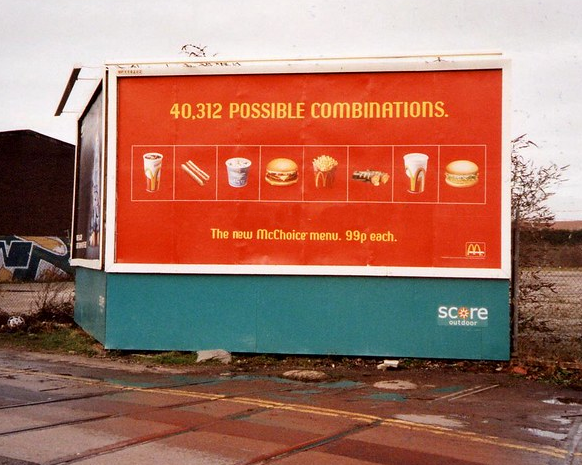
\includegraphics{img/mccombos.png}

}

\caption{\label{fig-mccombos}Una valla publicitaria anunciando el
lanzamiento del menú McChoice.}

\end{figure}

La elección de un menú específico surge de contestar ``sí'' o ``no'' a
ocho preguntas específicas: ¿quiere una gaseosa?, ¿quiere un pancho?,
¿quiere un helado?, etcétera. Como cada uno de los ítems son
distinguibles entre sí, la herramienta de conteo adecuada para este
problema es una permutación con repetición, porque se repite ocho veces
la pregunta de sí/no pero, dependiendo del orden en que se pregunta,
cada respuesta está asociada a un ítem diferente. En otras palabras, se
tiene un total de \(2^8 = 256\) menúes posibles, aunque lo correcto
sería excluir el caso del ``menú vacío'', donde el cliente contesta
``no'' a todas las preguntas (no tendría sentido). En ese caso el
resultado es: \[2^8 - 1 = 256 - 1 = 255 \text{ menúes posibles.}\]

¿Cómo McDonald's arribó a un número tan distinto? Se desconoce el
cálculo que realizaron, visto que públicamente negaron haber cometido un
error (Parker 2019), pero es fácil observar que \(40\,312 = 8! - 8.\)
Dada la similitud entre la estructura de este cálculo y la respuesta
correcta, es sensato suponer que McDonald's intentó seguir la misma
lógica. El mayor error que cometieron fue usar un número factorial, el
cual sirve para contar el número de formas de \emph{ordenar} los ocho
ítems del menú. Es decir, asumieron que los clientes pedirían todos los
ítems del menú y las ``diferencias'' entre ellos surgirían del orden en
que estos alimentos fuesen consumidos (si bien esto es ilógico porque,
por ejemplo, la gaseosa suele consumirse al mismo tiempo que la gaseosa,
en vez de antes o después).

Un total de 154 personas presentaron una queja oficial a la
\emph{Advertising Standards Authority} de Reino Unido. A pesar de estar
publicitando un número que resultó ser más de cien veces mayor al real,
la agencia falló a favor de McDonald's (Parker 2019). Desde entonces, se
le llaman McCombinaciones\footnote{Secuencia
  \href{https://oeis.org/A005096/internal}{A005096} de la OEIS.} a los
números del tipo \(n!-n\), donde para \(n=8\) se tiene el número
utilizado en la publicidad.

\bookmarksetup{startatroot}

\hypertarget{referencias}{%
\chapter*{Referencias}\label{referencias}}
\addcontentsline{toc}{chapter}{Referencias}

\markboth{Referencias}{Referencias}

\hypertarget{refs}{}
\begin{CSLReferences}{1}{0}
\leavevmode\vadjust pre{\hypertarget{ref-parker2019}{}}%
Parker, M. 2019. \emph{Humble Pi: A Comedy of Maths Errors}. Penguin
Books Limited. \url{https://books.google.com.ar/books?id=qYlZDwAAQBAJ}.

\end{CSLReferences}



\end{document}
